\chapter{Kendali Daur Sel dan Kematian Sel Terprogram}\label{ch:b3:cell-cycle-apoptosis}

Kira-kira seratus miliar sel tubuh Anda akan mati hari ini, dengan sengaja,
dan seratus miliar lagi akan lahir menggantikannya; lapisan usus Anda
diperbarui tiap lima hari, dan sel darah merah Anda tiap empat bulan.
Seekor berudu kehilangan ekornya tanpa berdarah; selaput di antara jari embrio
manusia lenyap pada minggu kedelapan; separuh neuron yang pernah dibuat di
dalam sebuah otak dibunuh sebelum kelahiran. Setiap kematian itu dilaksanakan
sel itu sendiri, menurut sebuah program, dan setiap kelahirannya diizinkan
sistem kendali yang memutuskan, pada dua atau tiga titik daurnya, apakah selnya
boleh melanjut. Kedua program itu --- pembelahan dan bunuh diri --- adalah
pokok bab ini. Keduanya dipecahkan pada khamir, telur katak, bulu babi, dan
seekor cacing yang bersel somatik tepat $1090$ dan tepat $131$ di antaranya
mati, lalu keduanya ternyata sama pada manusia, tempat kegagalannya menjadi
kanker di satu sisi dan kemunduran di sisi yang lain.

\section{Mesin daurnya}

\begin{definition}[Siklin dan kinase bergantung-siklin]\label{def:b3:cell-cycle-apoptosis:cdk}
\index{siklin}\index{kinase bergantung-siklin}%
\index{kompleks pemacu anafase}\index{daur sel}
Daur sel --- G1, S (replikasi), G2, M (mitosis) --- digerakkan sebuah famili
kinase protein, yaitu \emph{kinase bergantung-siklin} (CDK), yang subunit
katalitiknya hadir sepanjang daurnya tetapi hanya aktif ketika terikat pada
sebuah \emph{siklin}, yakni subunit pengatur yang kepekatannya naik lalu turun
menurut urutan yang tetap: siklin D bersama Cdk4/6 pada G1 sebagai tanggapan
atas faktor pertumbuhan, siklin E bersama Cdk2 pada peralihan G1/S, siklin A
bersama Cdk2 sepanjang S, dan siklin B bersama Cdk1 saat masuk mitosis. Tiap
siklin--CDK memfosforilasi protein fasenya --- titik asal replikasi, lamin,
kondensin, enzim perakitan gelendong --- dan masing-masing dimatikan oleh
pemusnahan siklinnya: ligase ubikuitin (SCF pada G1/S, \emph{kompleks pemacu
anafase}, APC/C, pada mitosis) menandai siklinnya bagi proteasom. Keaktifan
Cdk1 selanjutnya digerbangi sebuah fosforilasi penghambat yang dipasang kinase
Wee1 lalu dibuang fosfatase Cdc25, dan digerbangi protein penghambat kecil
(p21, p27, p16) yang mengikat kompleksnya. Daurnya dengan demikian merupakan
runtunan gelombang kinase yang teratur, dan tiap gelombangnya berakhir pada
proteolisis apa yang menghasilkannya.
\end{definition}

\begin{proof}[Bukti eksperimental]
Tiga jalur memusat. Hartwell (dasawarsa 1970-an) memisahkan mutan
\emph{cdc} khamir bertunas yang peka suhu, yang masing-masing terhenti pada
satu tahap dengan ukuran tunas yang khas, lalu menetapkan \emph{Start}, yakni
titik pada G1 yang sesudahnya sebuah sel terikat pada satu daur. Nurse
(dasawarsa 1980-an) mendapati pada khamir belah bahwa \emph{cdc2} mengendalikan
penataan waktu mitosisnya dan bahwa gen manusianya, yang dimasukkan ke dalam
khamirnya, menyelamatkan mutannya: kinasenya adalah Cdk1, yang lestari dari
khamir sampai manusia. Hunt (1983) mendapati pada telur bulu babi sebuah
protein yang menumpuk sepanjang tiap daurnya lalu dimusnahkan
mendadak pada tiap pembelahan, dan menamainya \omterm{def:b3:cell-cycle-apoptosis:cdk}{siklin}. Telur katak
sementara itu telah memberi ``faktor pemacu pematangan'' yang mendorong
nukleus mana pun masuk mitosis; faktor itu adalah \omterm{def:b3:cell-cycle-apoptosis:cdk}{siklin} B yang terikat pada
Cdk1. Rao dan Johnson (1970) sebelumnya telah menunjukkan lewat penggabungan
sel bahwa sel berfase S mendorong nukleus G1 masuk ke replikasi, sedangkan
nukleus G2 menunggu --- sitoplasmanya mengusung isyaratnya, dan nukleus yang
telah bereplikasi tak dapat dipaksa bereplikasi lagi.
\end{proof}

\begin{omfigure}
\begin{tikzpicture}[every node/.style={font=\scriptsize}, >=stealth]
  % cycle circle with phases
  \draw[very thick, omDef!50] (0,0) circle (2.2);
  \foreach \a/\b/\col/\lab/\r in {90/200/omDef!25/G1/1.55, 200/270/omProp!30/S/1.55, 270/315/omMeth!30/G2/1.55, 315/450/omThm!30/M/1.55} {
    \fill[\col] (0,0) -- (\a:2.2) arc[start angle=\a, end angle=\b, radius=2.2] -- cycle;
    \node[font=\small\bfseries] at ({(\a+\b)/2}:\r) {\lab};
  }
  \fill[white] (0,0) circle (1.0);
  \draw[very thick, omDef!50] (0,0) circle (2.2);
  % cyclin-CDK labels around
  \node[left, align=right] at (-2.4,1.2) {siklin D--Cdk4/6\\faktor pertumbuhan, Rb mati};
  \node[left, align=right] at (-2.4,-1.0) {siklin E--Cdk2\\titik asalnya menyala};
  \node[anchor=north east, align=right] at (-1.3,-2.2) {siklin A--Cdk2\\replikasi};
  \node[right, align=left] at (2.4,-1.0) {siklin B--Cdk1\\masuk ke mitosis};
  \node[right, align=left] at (2.4,1.3) {APC/C memusnahkan siklin B\\dan sekurin: anafase, keluar};
  % checkpoints as bars
  \foreach \a in {160,270,20} \draw[very thick, omThm] (\a:1.95) -- (\a:2.45);
  \node[align=center, anchor=south east] at (-1.2,2.35) {titik batas:\\adakah faktor pertumbuhan?};
  \node[align=left, anchor=west] at (2.55,0.35) {titik periksa gelendong:\\sudahkah semua kinetokor melekat?};
  \node[align=center, anchor=north] at (1.5,-2.55) {titik periksa G2/M:\\utuhkah DNA-nya?};
  \draw[->, thick] (0,0) ++(60:1.25) arc[start angle=60, end angle=30, radius=1.25];
\end{tikzpicture}

{\small Daurnya sebagai runtunan gelombang siklin--CDK, dan tiap gelombangnya
diakhiri pemusnahan \omterm{def:b3:cell-cycle-apoptosis:cdk}{siklinnya}, dengan ketiga \omterm{def:b3:cell-cycle-apoptosis:checkpoints}{titik periksanya} (batang merah)
tempat selnya bertanya apakah akan melanjut.}
\end{omfigure}

\begin{theorem}[Sebuah sakelar dan sebuah rem yang tertunda membuat osilator]\label{thm:b3:cell-cycle-apoptosis:oscillator}
\index{osilator relaksasi}\index{kedwimantapan!daur sel}\index{histeresis}
Misalkan $A$ adalah keaktifan \omterm{def:b3:cell-cycle-apoptosis:cdk}{siklin} B--Cdk1 dan $C$ adalah jumlah \omterm{def:b3:cell-cycle-apoptosis:cdk}{siklin}
B. Andaikan (i) untuk $C$ yang tetap, $A$ melemas dengan cepat ke sebuah
keadaan tunak yang bergantung pada $C$ lewat umpan balik positif (Cdk1 aktif
mengaktifkan pengaktifnya Cdc25 dan menghambat penghambatnya Wee1), sehingga
kurva keadaan tunaknya $A^{*}(C)$ berbentuk S: untuk $C$ di antara dua
ambang $C_{1} < C_{2}$ terdapat keadaan rendah maupun keadaan tinggi, dan
sistemnya bertahan pada cabang mana pun yang sedang ditempatinya
(\emph{histeresis}); (ii) $C$ berubah perlahan, disintesis dengan laju tetap
$k_{s}$ lalu diuraikan dengan laju $k_{d}A\,C$ lewat APC/C, yang dinyalakan
Cdk1 aktif sesudah sebuah tundaan. Maka sistemnya tak memiliki keadaan tunak
yang mantap lalu menjalankan sebuah \emph{osilasi relaksasi}: $C$ menumpuk
pada cabang rendahnya sampai melewati $C_{2}$, $A$ melompat ke cabang
tingginya (masuknya mitosis), penguraiannya melampaui sintesisnya dan $C$
turun sampai melewati $C_{1}$, $A$ runtuh ke cabang rendahnya (keluarnya
mitosis), lalu daurnya berulang. Periodenya terutama ditentukan variabel yang
lambat: kira-kira $C_{2}/k_{s}$ bagi kenaikannya, ditambah waktu menguraikan
dari $C_{2}$ ke $C_{1}$.
\end{theorem}
\begin{proof}[Bukti sebagian]
Sebuah keadaan tunak pasangan itu akan menuntut $\mathrm{d}C/\mathrm{d}t = 0$,
yakni $k_{s} = k_{d}A^{*}(C)\,C$, pada sebuah titik di kurva berbentuk S itu.
Pada cabang rendahnya $A^{*}$ kecil, sehingga $k_{d}A^{*}C < k_{s}$ untuk $C$
sampai $C_{2}$: \omterm{def:b3:cell-cycle-apoptosis:cdk}{siklinnya} naik, dan sistemnya terbawa keluar dari ujung
cabangnya. Pada cabang tingginya $A^{*}$ besar, sehingga $k_{d}A^{*}C > k_{s}$
untuk $C$ turun sampai $C_{1}$: \omterm{def:b3:cell-cycle-apoptosis:cdk}{siklinnya} turun, dan sistemnya terbawa keluar
dari ujung itu. Satu-satunya calon keadaan tunaknya akan terletak pada cabang
tengahnya yang tak mantap, dan sebuah titik di situ menolak; jadi tak ada
keadaan tunak yang mantap, dan lintasannya, yang terkurung pada kedua cabang
mantapnya serta lompatan di antaranya, berdaur. Waktu pada cabang rendahnya
adalah $\int \mathrm{d}C/(k_{s} - k_{d}A^{*}C) \approx C_{2}/k_{s}$ ketika
$A^{*}$ kecil, dan waktu pada cabang tingginya adalah waktu yang lebih pendek
untuk menguraikan $C_{2} - C_{1}$ dengan laju $k_{d}A^{*}_{\text{tinggi}}C$.
Adanya kurva berbentuk S dari umpan balik Cdc25/Wee1 diterima tanpa bukti di
sini; kurva itu kedwimantapan yang sama dengan gen yang mengaktifkan dirinya
sendiri pada jilid Tahun~2, dengan variabel cepatnya kini sebuah kinase dan
variabel lambatnya \omterm{def:b3:cell-cycle-apoptosis:cdk}{siklinnya}.
\end{proof}

\begin{omfigure}
\begin{tikzpicture}
\begin{axis}[
  width=6.6cm, height=5.6cm,
  axis lines=left,
  xmin=0, xmax=1.4, ymin=0, ymax=1.1,
  xlabel={siklin B, $C$}, ylabel={keaktifan Cdk1, $A$},
  xlabel style={font=\small, at={(axis description cs:0.5,-0.12)}, anchor=north}, ylabel style={font=\small},
  tick label style={font=\scriptsize}, xtick={0.4,1.0}, xticklabels={$C_{1}$,$C_{2}$}, ytick=\empty,
  clip=false,
]
% S-shaped nullcline: two stable branches and a dashed unstable one
\addplot[very thick, omDef, smooth] coordinates {(0,0.02) (0.5,0.04) (0.9,0.07) (1.0,0.1)};
\addplot[very thick, omDef, dashed, smooth] coordinates {(1.0,0.1) (0.85,0.3) (0.7,0.5) (0.55,0.7) (0.4,0.9)};
\addplot[very thick, omDef, smooth] coordinates {(0.4,0.9) (0.6,0.94) (1.0,0.97) (1.4,0.98)};
\draw[->, very thick, omThm] (axis cs:0.05,0.15) -- (axis cs:0.98,0.15);
\draw[->, very thick, omThm] (axis cs:1.04,0.18) -- (axis cs:1.04,0.82);
\draw[->, very thick, omThm] (axis cs:0.98,0.84) -- (axis cs:0.42,0.84);
\draw[->, very thick, omThm] (axis cs:0.36,0.82) -- (axis cs:0.36,0.18);
\node[font=\scriptsize, omThm, anchor=south west] at (axis cs:0.36,0.24) {siklin menumpuk};
\node[font=\scriptsize, omThm, anchor=west] at (axis cs:1.07,0.5) {masuk};
\node[font=\scriptsize, omThm, anchor=south] at (axis cs:0.7,1.0) {APC/C menguraikan siklin (mitosis)};
\node[font=\scriptsize, omThm, anchor=east] at (axis cs:0.33,0.5) {keluar};
\node[font=\scriptsize, omDef, anchor=north east] at (axis cs:1.38,0.95) {$A^{*}(C)$};
\end{axis}
\begin{axis}[
  at={(7.6cm,0)}, anchor=south west,
  width=6.6cm, height=5.6cm,
  axis lines=left,
  xmin=0, xmax=3, ymin=0, ymax=1.2,
  xlabel={waktu (daur)}, ylabel={},
  xlabel style={font=\small, at={(axis description cs:0.5,-0.12)}, anchor=north},
  tick label style={font=\scriptsize}, xtick={0,1,2,3}, ytick=\empty,
  clip=false,
]
\addplot[very thick, omDef] coordinates {(0,0.4) (0.8,1.0) (0.95,0.4) (1.75,1.0) (1.9,0.4) (2.7,1.0) (2.85,0.4) (3,0.5)};
\addplot[very thick, omThm] coordinates {(0,0.05) (0.8,0.05) (0.8,0.95) (0.95,0.95) (0.95,0.05) (1.75,0.05) (1.75,0.95) (1.9,0.95) (1.9,0.05) (2.7,0.05) (2.7,0.95) (2.85,0.95) (2.85,0.05) (3,0.05)};
\node[font=\scriptsize, omDef, anchor=south west] at (axis cs:1.0,0.1) {siklin B};
\node[font=\scriptsize, omThm, anchor=south west] at (axis cs:1.0,1.0) {keaktifan Cdk1};
\end{axis}
\end{tikzpicture}

{\small Kiri: bidang fase osilatornya. Kurva berbentuk S itu adalah
keadaan tunak cepat Cdk1 bagi tiap kadar \omterm{def:b3:cell-cycle-apoptosis:cdk}{siklin}; gelung merahnya adalah
daurnya --- penumpukan lambat sepanjang cabang rendahnya, sebuah lompatan pada
$C_{2}$, penguraian cepat sepanjang cabang tingginya, dan lompatan kembali pada
$C_{1}$. Kanan: perjalanan waktu yang dihasilkannya, yakni gigi gergaji \omterm{def:b3:cell-cycle-apoptosis:cdk}{siklin}
dan gelombang kotak kinasenya.}
\end{omfigure}

\begin{example}[Mengapa telur katak adalah sebuah jam]\label{ex:b3:cell-cycle-apoptosis:frog}
Sebutir telur katak yang telah dibuahi membelah dua belas kali dalam enam jam
tanpa pertumbuhan, tanpa transkripsi, dan tanpa \omterm{def:b3:cell-cycle-apoptosis:checkpoints}{titik periksa}, pada selang
\qty{30}{min}: itulah osilator teoremanya yang berjalan telanjang, dan sebuah
ekstrak sitoplasmanya di dalam tabung reaksi terus berdaur, dengan \omterm{def:b3:cell-cycle-apoptosis:cdk}{siklinnya}
naik dan turun, tanpa apa pun yang dibelah. Menambahkan \omterm{def:b3:cell-cycle-apoptosis:cdk}{siklin} B yang tak
dapat diuraikan mengunci ekstraknya di dalam mitosis, karena $C$ tak pernah
dapat turun di bawah $C_{1}$; menghalangi sintesis \omterm{def:b3:cell-cycle-apoptosis:cdk}{siklinnya} menguncinya di
dalam interfase. Di dalam sel somatik, mesin yang sama terbungkus kendali
bagian berikutnya, yang menahannya pada ambangnya sampai syaratnya terpenuhi,
sehingga periodenya menjadi sehari alih-alih setengah jam dan dapat panjang
tanpa batas.
\end{example}

\section{Titik periksa}

\begin{definition}[Titik periksa]\label{def:b3:cell-cycle-apoptosis:checkpoints}
\index{titik periksa}\index{titik batas}%
\index{titik periksa perakitan gelendong}\index{pemberian izin replikasi}
Sebuah \emph{titik periksa} adalah kendali yang menghentikan daurnya pada
sebuah peralihan sampai sebuah syarat terpenuhi, dengan bekerja pada mesinnya
--- menghambat sebuah CDK atau sebuah ligase ubikuitin. Tiga di antaranya
paling penting. \emph{Titik batas} pada G1 akhir (Start pada khamir): selnya
melanjut hanya bila faktor pertumbuhan, hara, dan ukurannya mengizinkan; di
seberangnya daurnya rampung tanpa semua itu. \emph{Titik periksa G2/M}: DNA
yang rusak atau belum bereplikasi, yang diisyaratkan kinase \omterm{def:b3:dna-repair:ddr}{ATM}/ATR
\cref{ch:b3:dna-repair}, menjaga Cdc25 tetap terhambat sehingga menjaga Cdk1
tetap terfosforilasi dan tak aktif. \emph{Titik periksa perakitan gelendong}:
satu kinetokor saja yang tak melekat pada \omterm{def:b3:cytoskeleton-motility:filaments}{mikrotubulus} menghasilkan penghambat
yang dapat berdifusi (Mad2 yang terikat pada Cdc20) yang menjaga APC/C tetap
mati, sehingga anafasenya menunggu kromosom yang terakhir. Sebuah kendali
keempat tak memiliki langkah menunggu tetapi sama ketatnya: \emph{pemberian
izin replikasi}. Titik asalnya dimuati helikase MCM hanya pada G1, ketika
keaktifan CDK-nya rendah, dan faktor pemuatnya dimusnahkan atau dihambat
begitu fase S mulai, sehingga tiap titik asalnya menyala sekali dan hanya
sekali tiap daurnya --- itulah sebabnya nukleus G2 pada penggabungan Rao dan
Johnson tak dapat dipaksa bereplikasi.
\end{definition}

\begin{proposition}[Titik batas adalah sebuah sakelar]\label{prop:b3:cell-cycle-apoptosis:rb}
\index{protein retinoblastoma}\index{E2F}
Pada G1 awal faktor transkripsi \emph{E2F}, yang menggerakkan gen
fase S (\omterm{def:b3:cell-cycle-apoptosis:cdk}{siklin} E, \omterm{def:b3:cell-cycle-apoptosis:cdk}{siklin} A, enzim replikasinya), ditahan tak aktif oleh
\emph{\omterm{prop:b3:cell-cycle-apoptosis:rb}{protein retinoblastoma}} Rb. Faktor pertumbuhan mengimbas
\omterm{def:b3:cell-cycle-apoptosis:cdk}{siklin} D, lalu \omterm{def:b3:cell-cycle-apoptosis:cdk}{siklin} D--Cdk4/6 mulai memfosforilasi Rb sehingga melepaskan
sedikit E2F; E2F lalu mengimbas \omterm{def:b3:cell-cycle-apoptosis:cdk}{siklin} E, dan \omterm{def:b3:cell-cycle-apoptosis:cdk}{siklin} E--Cdk2 memfosforilasi
Rb jauh lebih banyak --- yakni umpan balik positif yang, sekali melewati
sebuah ambang, menuntaskan dirinya sendiri tanpa faktor pertumbuhan lagi.
Selnya telah menyeberangi \omterm{def:b3:cell-cycle-apoptosis:checkpoints}{titik batasnya}; E2F juga mengimbas gennya sendiri.
Hilangnya Rb, atau hilangnya penghambat Cdk4/6 bernama p16, atau penguatan
\omterm{def:b3:cell-cycle-apoptosis:cdk}{siklin} D, sama sekali menghapus tuntutan akan faktor pertumbuhan, dan
masing-masing lazim pada kanker (\cref{ch:b3:cancer-biology}); obat yang
menghambat Cdk4/6 kini dipakai melawan kanker payudara yang bergantung pada
sakelar ini.
\end{proposition}

\begin{omfigure}
\begin{tikzpicture}[every node/.style={font=\scriptsize}, >=stealth]
  \node[draw, thick, rounded corners, fill=omProp!25, minimum width=2.2cm] (gf) at (0,2.2) {faktor pertumbuhan};
  \node[draw, thick, rounded corners, fill=omDef!20, minimum width=2.4cm] (cd) at (0,1.0) {siklin D--Cdk4/6};
  \node[draw, thick, rounded corners, fill=omThm!20, minimum width=1.6cm] (rb) at (3.8,1.0) {Rb};
  \node[draw, thick, rounded corners, fill=omMeth!25, minimum width=1.6cm] (e2f) at (7.2,1.0) {E2F};
  \node[draw, thick, rounded corners, fill=omDef!20, minimum width=2.4cm] (ce) at (7.2,-0.6) {siklin E--Cdk2};
  \node[draw, thick, rounded corners, fill=gray!15, align=center, minimum width=2.6cm] (s) at (10.8,1.0) {gen fase S:\\siklin A, MCM, \dots};
  \draw[->, thick] (gf) -- (cd);
  \draw[-|, thick, omThm] (cd) -- (rb) node[midway, above, font=\tiny] {memfosforilasi};
  \draw[-|, thick, omThm] (rb) -- (e2f) node[midway, above, font=\tiny] {menahannya tak aktif};
  \draw[->, thick] (e2f) -- (s);
  \draw[->, thick] (e2f) -- (ce) node[midway, right] {mengimbas};
  \draw[-|, thick, omThm] (ce.west) -- ++(-2.2,0) |- (rb.south) node[pos=0.25, below] {memfosforilasi Rb lebih lanjut};
  \draw[->, thick, omMeth!70!black] (e2f.north) .. controls (6.0,2.2) and (6.8,2.2) .. (e2f.north east) node[pos=0.5, above] {mengimbas gennya sendiri};
  \node[draw, thick, rounded corners, fill=omThm!10] (p16) at (0,-0.6) {p16}; \draw[-|, thick, omThm] (p16) -- (cd);
\end{tikzpicture}

{\small \omterm{def:b3:cell-cycle-apoptosis:checkpoints}{Titik batasnya}. Faktor pertumbuhan memulai fosforilasi
Rb, yang membebaskan sedikit E2F; E2F mengimbas \omterm{def:b3:cell-cycle-apoptosis:cdk}{siklin} E, yang kinasenya
memfosforilasi Rb lebih lanjut --- yakni umpan balik positif yang menuntaskan
peralihannya lalu membuatnya tak bergantung pada isyarat awalnya. Batangnya
menandai penghambatan.}
\end{omfigure}

\begin{proposition}[Anafase adalah keputusan proteolitik]\label{prop:b3:cell-cycle-apoptosis:anaphase}
\index{sekurin}\index{separase}\index{kohesin}
Kromatid saudari ditahan bersama sejak fase S oleh cincin
\emph{kohesin}. Pada metafase, ketika tiap kinetokornya telah melekat dan
\omterm{def:b3:cell-cycle-apoptosis:checkpoints}{titik periksa} gelendongnya dibungkam, APC/C bersama pengaktifnya Cdc20
mengubikuitinasi dua protein: \omterm{def:b3:cell-cycle-apoptosis:cdk}{siklin} B, yang hilangnya menonaktifkan Cdk1 dan
memungkinkan selnya keluar dari mitosis, dan \emph{sekurin}, yang hilangnya
membebaskan protease \emph{separase}, yang memotong kohesinnya. Semua pasangan
saudarinya memisah dalam hitungan detik satu sama lain, ditarik ke kutubnya
oleh gelendongnya, lalu selnya membelah dengan sebuah cincin aktin dan
\omterm{def:b3:cytoskeleton-motility:motors}{miosin}~II yang dirakit di tempat yang diberitahukan zona tengah gelendongnya
kepada korteksnya (lewat RhoA). Keputusannya tak berbalik karena keputusan itu
proteolitik: kohesin yang terpotong tak dapat dirakit kembali, dan \omterm{def:b3:cell-cycle-apoptosis:cdk}{siklin} yang
telah diuraikan harus disintesis ulang. Galat di sini --- sebuah kromosom yang
ditarik ke kutub yang keliru, sebuah anafase yang dimulai sebelum pelekatan
terakhirnya --- menghasilkan sel anak yang aneuploid, yakni kelainan kromosom
yang paling lazim pada tumor dan pada keguguran.
\end{proposition}

\begin{omfigure}
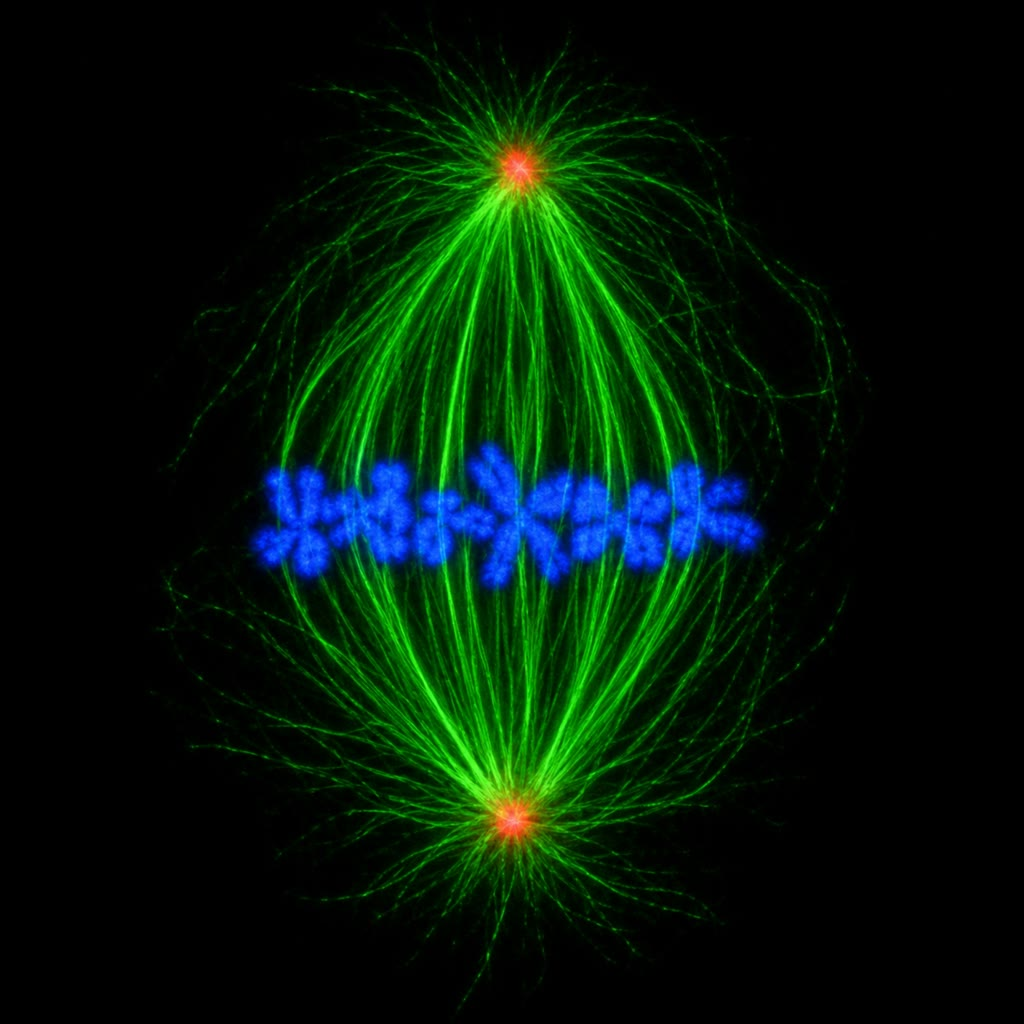
\includegraphics[width=0.36\linewidth]{images/book5/ai/b5-10-mitotic-spindle.jpg}\hspace{0.04\linewidth}
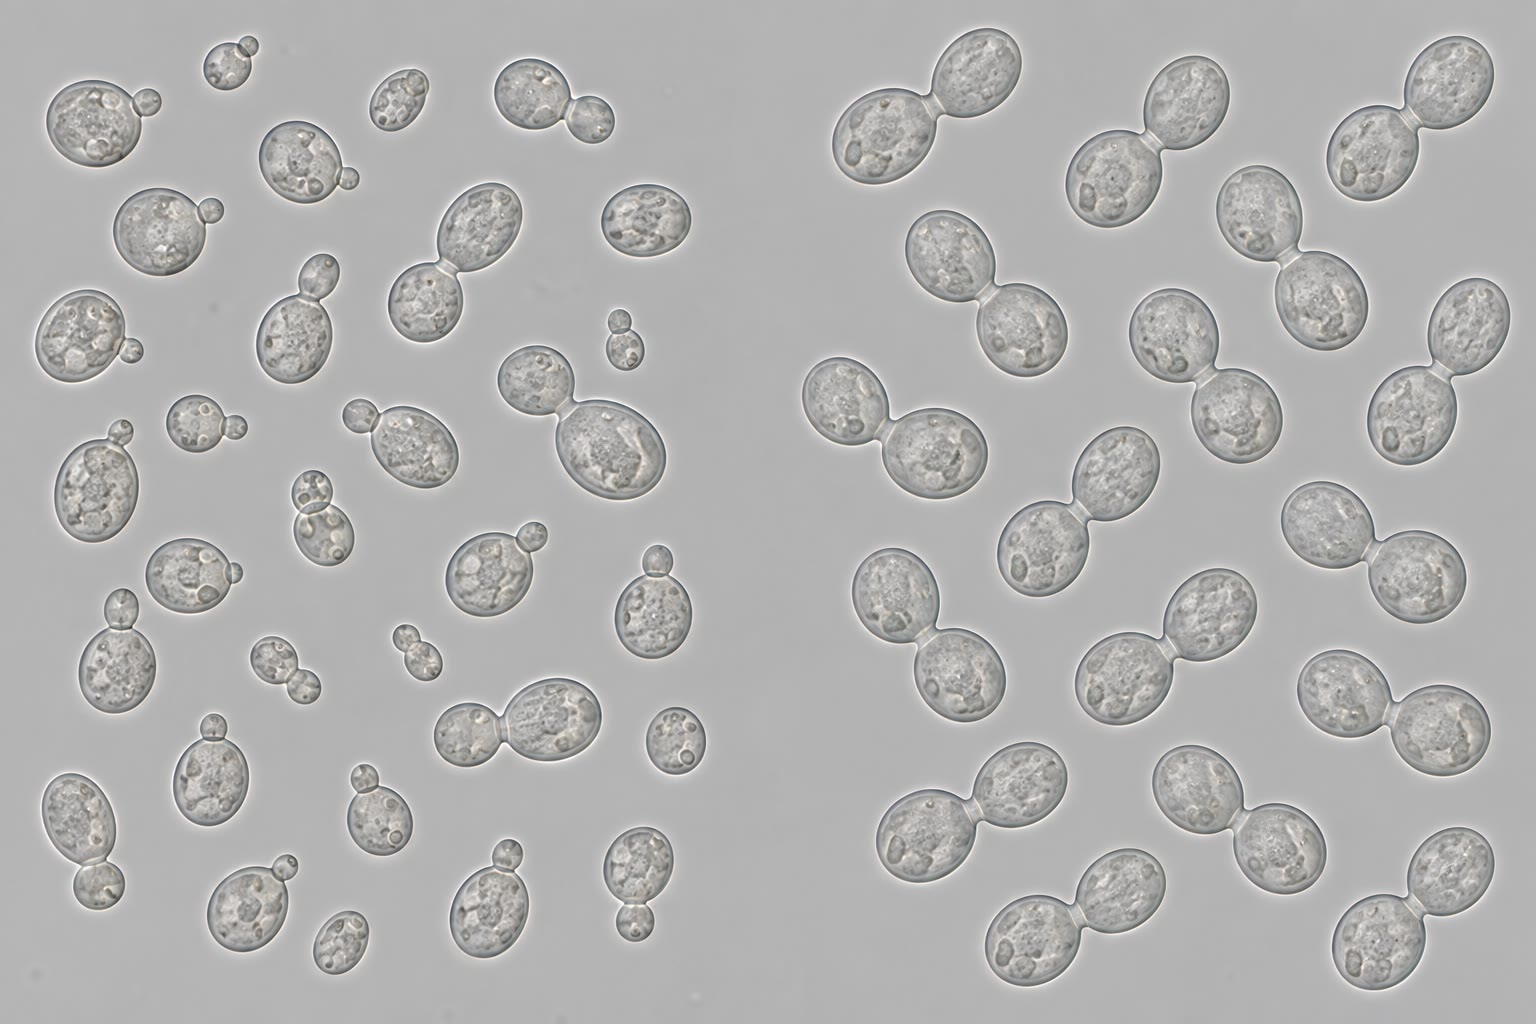
\includegraphics[width=0.54\linewidth]{images/book5/ai/b5-10-yeast-cdc-mutants.jpg}

{\small Kiri: sebuah sel metafase --- \omterm{def:b3:cytoskeleton-motility:filaments}{mikrotubulus} gelendong (hijau) dari
kedua kutubnya (merah), kromosom (biru) yang berbaris pada pelatnya, yakni
saat ketika \omterm{def:b3:cell-cycle-apoptosis:checkpoints}{titik periksa} gelendongnya memutuskan. Kanan: khamir bertunas,
tipe liar dengan tunas beraneka ukuran (kiri) dan sebuah mutan \emph{cdc}
yang setiap selnya terhenti pada tahap yang sama, masing-masing dengan tunas
berukuran sama (kanan).}
\end{omfigure}

\section{Apoptosis}

\begin{definition}[Apoptosis]\label{def:b3:cell-cycle-apoptosis:apoptosis}
\index{apoptosis}\index{nekrosis}\index{kaspase}\index{fosfatidilserina}
\emph{Apoptosis} adalah kematian sel terprogram lewat runtunan intrinsik:
selnya mengerut dan membulat, \omterm{def:b3:chromatin-epigenetics:nucleosome}{kromatinnya} memadat dan DNA-nya dipotong
di antara \omterm{def:b3:chromatin-epigenetics:nucleosome}{nukleosom} menjadi tangga fragmen, nukleusnya pecah,
membrannya menggelembung menjadi vesikel yang tersegel, fosfatidilserina
muncul pada muka luar membrannya sebagai isyarat ``makanlah aku'', dan
pecahannya ditelan tetangganya atau makrofag dalam waktu sejam ---
tanpa rembesan, dan karena itu tanpa peradangan. Semuanya dilaksanakan
\emph{kaspase}, yakni protease sisteina yang memotong sesudah aspartat, yang
dibuat sebagai zimogen tak aktif: kaspase \emph{pemrakarsa} (8 dan 9)
diaktifkan dengan dikumpulkan pada sebuah panggung, lalu keduanya memotong dan
mengaktifkan kaspase \emph{algojo} (3 dan 7), yang memotong beberapa ratus
substrat --- laminnya, sitoskeletonnya, penghambat nuklease pemotong DNA-nya,
serta enzim yang menjaga fosfatidilserina tetap di dalam.
\emph{Nekrosis}, sebaliknya, adalah kematian karena cedera: selnya membengkak,
pecah, menumpahkan isinya, lalu menimbulkan peradangan. Apoptosis dinamai dan
morfologinya diuraikan Kerr, Wyllie, dan Currie (1972);
gennya ditemukan pada seekor cacing.
\end{definition}

\begin{proof}[Bukti eksperimental]
Tiap hermafrodit \emph{Caenorhabditis elegans} membuat $1090$ sel somatik,
dan $131$ sel yang sama di antaranya mati, masing-masing pada waktu dan tempat
yang tetap. Horvitz dan rekan (dasawarsa 1980-an) memisahkan mutan yang
sel-sel itu justru bertahan hidup: \emph{ced-3} dan \emph{ced-4} dibutuhkan
bagi tiap kematiannya, dan tanpa keduanya ke-$131$ sel itu hidup lalu
berdiferensiasi; \emph{ced-9} melindungi --- hilangnya membunuh sel yang
semestinya hidup, keaktifannya yang berlebih menyelamatkan sel yang semestinya
mati; \emph{egl-1} dibutuhkan bagi kematian tertentu. CED-3 adalah sebuah
\omterm{def:b3:cell-cycle-apoptosis:apoptosis}{kaspase}, CED-4 panggung pengaktifnya (Apaf-1 pada manusia), CED-9 sebuah
protein Bcl-2, dan EGL-1 sebuah protein BH3 saja: yakni jalur manusianya, gen
demi gen. Gen \emph{BCL2} manusianya sendiri telah ditemukan pada sebuah
translokasi kromosom pada limfoma folikular, yakni kanker sel yang gagal mati.
\end{proof}

\begin{definition}[Kedua jalurnya]\label{def:b3:cell-cycle-apoptosis:pathways}
\index{jalur intrinsik}\index{jalur ekstrinsik}\index{famili Bcl-2}%
\index{sitokrom c}\index{apoptosom}\index{reseptor kematian}
Jalur \emph{intrinsik} (mitokondria) memadukan keadaan dalam sebuah sel.
\emph{Famili Bcl-2} memiliki tiga golongan: penjaga
(Bcl-2, Bcl-xL, Mcl-1) yang duduk pada membran luar mitokondria lalu
menjaganya tetap tersegel; efektor (Bax, Bak) yang, begitu diaktifkan,
mengoligomerisasi menjadi pori pada membran itu; dan pengindera \emph{BH3
saja} (Bim, Bid, Puma, Noxa, Bad), yang masing-masing diimbas atau diaktifkan
sebuah hinaan tertentu --- kerusakan DNA lewat p53 (Puma, Noxa), hilangnya
faktor pertumbuhan (Bim, Bad), terlepasnya pelekatan, protein yang salah
lipat --- yang mengikat penjaganya lalu membebaskan atau mengaktifkan
efektornya. Ketika efektornya menang, membran luarnya dipermeabilisasi,
\emph{sitokrom~c} merembes ke dalam sitosol, mengikat Apaf-1 lalu membentuk
\emph{apoptosom}, yang mengaktifkan \omterm{def:b3:cell-cycle-apoptosis:apoptosis}{kaspase}~9. Jalur
\emph{ekstrinsik} mulai dari luar: \emph{reseptor kematian} (Fas,
reseptor TNF, reseptor TRAIL) yang diikat ligannya pada sebuah limfosit
pembunuh atau pada tetangganya, mengelompok, merekrut adaptor, lalu
mengaktifkan \omterm{def:b3:cell-cycle-apoptosis:apoptosis}{kaspase}~8, yang memotong \omterm{def:b3:cell-cycle-apoptosis:apoptosis}{kaspase}~3 secara langsung dan, lewat
Bid, juga membuka rute mitokondrianya. Kedua jalurnya memusat pada
\omterm{def:b3:cell-cycle-apoptosis:apoptosis}{kaspase} algojonya, dan protein penghambat (IAP, FLIP) menetapkan
ambangnya di sepanjang jalan.
\end{definition}

\begin{omfigure}
\begin{tikzpicture}[every node/.style={font=\scriptsize}, >=stealth]
  % extrinsic
  \node[draw, thick, rounded corners, fill=omProp!25, align=center] (lig) at (0,4.2) {ligan kematian pada sel pembunuh\\(FasL, TNF, TRAIL)};
  \node[draw, thick, rounded corners, fill=omProp!25, align=center] (rec) at (0,2.8) {reseptor kematiannya mengelompok;\\adaptornya merekrut kaspase-8};
  \node[draw, thick, rounded corners, fill=omThm!20] (c8) at (0,1.5) {kaspase-8 aktif};
  % intrinsic
  \node[draw, thick, rounded corners, fill=omDef!20, align=center] (insult) at (7.2,4.2) {kerusakan DNA (p53), hilangnya faktor pertumbuhan,\\lepasnya pelekatan, dan protein yang salah lipat};
  \node[draw, thick, rounded corners, fill=omDef!20, align=center] (bh3) at (7.2,3.0) {pengindera BH3 saja (Puma, Bim, Bid)\\menetralkan Bcl-2, mengaktifkan Bax/Bak};
  \node[draw, thick, rounded corners, fill=omDef!20, align=center] (mito) at (7.2,1.7) {membran luar mitokondria membuka:\\sitokrom $c$ keluar, apoptosom terbentuk};
  \node[draw, thick, rounded corners, fill=omThm!20] (c9) at (7.2,0.5) {kaspase-9 aktif};
  % convergence
  \node[draw, thick, rounded corners, fill=omThm!35, align=center] (c3) at (3.6,-0.8) {kaspase algojo 3 dan 7:\\ratusan substrat dipotong};
  \node[draw, thick, rounded corners, fill=gray!15, align=center] (out) at (3.6,-2.3) {kromatin memadat, DNA bertangga, menggelembung,\\fosfatidilserina terpapar, lalu ditelan};
  \draw[->, thick] (lig) -- (rec); \draw[->, thick] (rec) -- (c8); \draw[->, thick] (c8) -- (c3);
  \draw[->, thick] (insult) -- (bh3); \draw[->, thick] (bh3) -- (mito); \draw[->, thick] (mito) -- (c9); \draw[->, thick] (c9) -- (c3);
  \draw[->, thick] (c3) -- (out);
  \draw[->, thick, dashed] (c8) -- (bh3) node[pos=0.55, below, sloped] {Bid terpotong: kedua rutenya bergabung};
  \node[left, omThm, align=right] at (-2.3,1.5) {jalur\\ekstrinsik}; \node[right, omDef, align=left] at (10.4,1.7) {jalur\\intrinsik};
  \node[right, font=\tiny, align=left] at (8.6,0.5) {IAP menghambat di sini;\\Bcl-2 menjaga di atasnya};
\end{tikzpicture}

{\small Kedua rute menuju \omterm{def:b3:cell-cycle-apoptosis:apoptosis}{kaspase} algojonya. Dari luar ke dalam, sebuah
\omterm{def:b3:cell-cycle-apoptosis:pathways}{reseptor kematian} mengaktifkan kaspase-8; dari dalam ke luar, \omterm{def:b3:cell-cycle-apoptosis:pathways}{famili Bcl-2}
menimbang keadaan selnya dan, ketika efektornya menang, mitokondrianya
melepaskan sitokrom~$c$ lalu kaspase-9 diaktifkan. Keduanya memusat pada kaspase-3.}
\end{omfigure}

\begin{proposition}[Titik tanpa kembali]\label{prop:b3:cell-cycle-apoptosis:mompt}
\index{permeabilisasi membran luar mitokondria}
\omterm{prop:b3:cell-cycle-apoptosis:mompt}{Permeabilisasi membran luar mitokondria} berlangsung mendadak
--- seluruh mitokondria sebuah sel membuka dalam kira-kira lima menit,
sesudah berjam-jam pertimbangan --- dan tuntas: begitu sitokrom~$c$ berada
di dalam sitosol, pengaktifan \omterm{def:b3:cell-cycle-apoptosis:apoptosis}{kaspase} menyusul dalam hitungan menit dan tak
dapat dibatalkan dengan membuang rangsangannya. Dua ciri menjadikannya sebuah
sakelar. Pori Bax/Bak terbentuk lewat oligomerisasi, sehingga lajunya naik
tajam terhadap jumlah efektor yang teraktifkan; dan penjaganya serta
penginderanya saling mengikat dengan kegemaran tinggi, sehingga sampai sebuah
ambang tiap penginderanya ternetralkan dan di seberangnya tiap pengindera
tambahan menjadi bebas --- yakni sebuah titrasi, seperti dapar yang terkuras.
Karena itu selnya tidak mati berangsur; ia menimbun protein BH3 saja sampai
sebuah ambang terlewati, lalu mati sekaligus. Obat yang meniru protein BH3
(venetoklaks, yang menduduki Bcl-2) mendorong sel yang ``tersiap'' ---
yakni yang sudah dekat ambangnya, sebagaimana banyak sel leukemia ---
melewatinya, sambil mengampuni sel yang tidak.
\end{proposition}

\begin{omfigure}
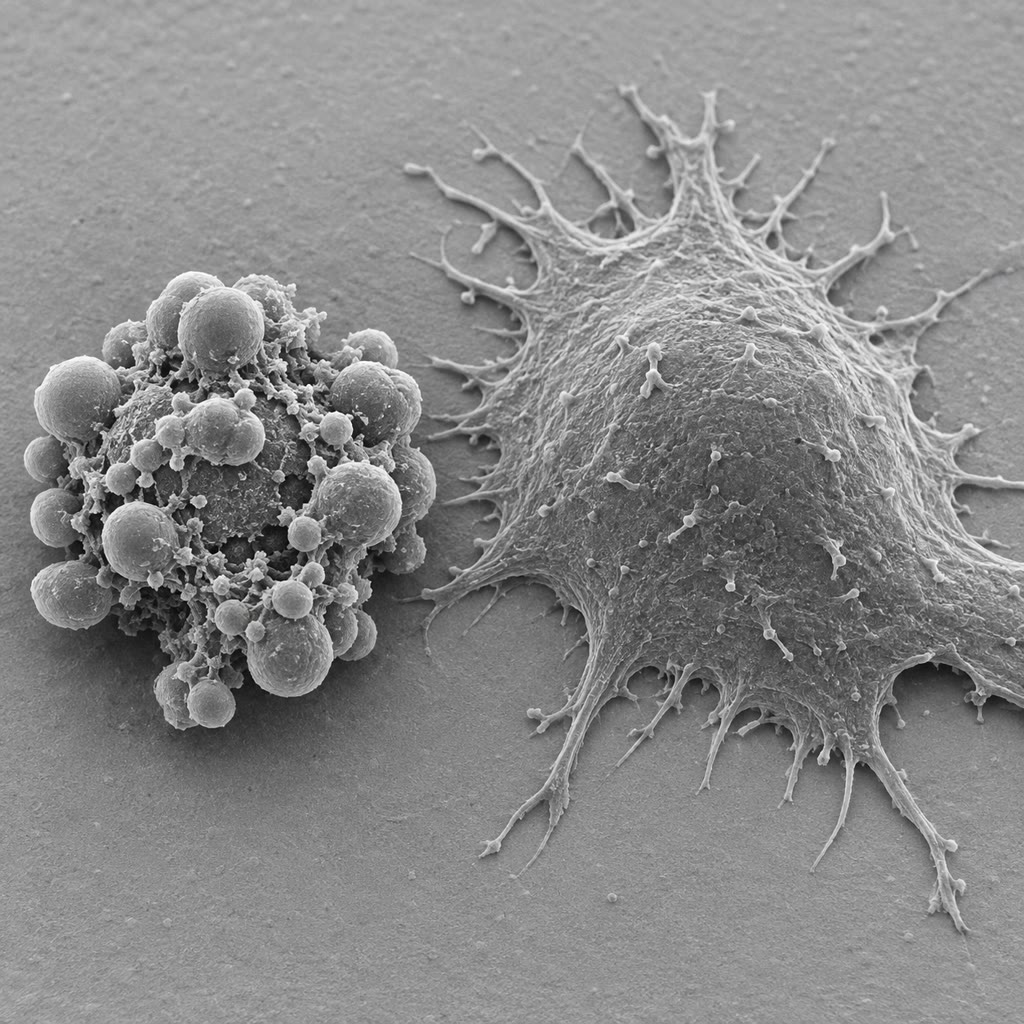
\includegraphics[width=0.40\linewidth]{images/book5/ai/b5-10-apoptotic-cell.jpg}

{\small Sebuah sel apoptotik di samping sel yang sehat di bawah mikroskop
elektron payar: mengerut, dengan permukaannya pecah menjadi gelembung tersegel
yang akan ditelan tanpa jejak peradangan.}
\end{omfigure}

\begin{example}[Kematian yang membangun sebuah tubuh]\label{ex:b3:cell-cycle-apoptosis:development}
Jari diukir dari sebuah dayung oleh \omterm{def:b3:cell-cycle-apoptosis:apoptosis}{apoptosis} sel di antaranya;
pada bebek sel yang sama justru hidup dan selaputnya bertahan.
Ekor berudu diserap kembali saat metamorfosis atas isyarat hormon
tiroid. Kira-kira separuh neuron yang dihasilkan sistem saraf vertebrata
mati sebelum kelahiran, yakni neuron yang gagal menerima cukup faktor trofik
dari sasarannya --- sebuah persaingan yang menyerasikan cacah neuronnya dengan
luas medan yang dilayaninya. Sembilan puluh lima persen sel~T yang dibuat di
dalam timus mati di situ, tersaring keluar karena tidak mengenali apa pun atau
karena mengenali dirinya sendiri (\cref{ch:b3:adaptive-immunity}).
Dan setiap hari epitelium usus melepaskan sel tertuanya pada puncak vilinya,
kulit melepaskan keratinositnya, darah melepaskan neutrofil tuanya sesudah
hidup sehari: \omterm{def:b3:cell-cycle-apoptosis:apoptosis}{apoptosis} adalah kelaziman, dan ukuran sebuah jaringan
adalah selisih dua laju yang besar.
\end{example}

\section{Jalan keluar yang lain, dan kegagalan keluar}

\begin{definition}[Nekrosis terkendali dan penuaan sel]\label{def:b3:cell-cycle-apoptosis:other}
\index{nekroptosis}\index{piroptosis}\index{penuaan sel}
Sel memiliki kematian terprogram yang lain, dan semuanya membangkitkan
peradangan sedangkan \omterm{def:b3:cell-cycle-apoptosis:apoptosis}{apoptosis} membisu. \emph{Nekroptosis}, yang dipicu
\omterm{def:b3:cell-cycle-apoptosis:pathways}{reseptor kematian} ketika kaspase-8 terhalang (sebagaimana sebagian virus
menghalanginya), merakit kinase RIPK3 bersama MLKL, yang melubangi membran
plasmanya. \emph{Piroptosis}, di dalam makrofag yang terinfeksi, dilaksanakan
kaspase-1 milik inflamasom (\cref{ch:b3:innate-immunity}), yang memotong
gasdermin menjadi pembentuk pori lalu melepaskan interleukin-1.
\emph{Feroptosis} adalah kematian lewat peroksidasi lipid yang bergantung
besi. Sebuah sel juga dapat berhenti membelah tanpa mati: \emph{penuaan sel}
adalah penghentian yang permanen, yang dipaksakan p16 dan p21 sesudah
pengikisan telomer (\cref{ch:b3:stem-cells}), kerusakan DNA yang bertahan,
atau pengaktifan onkogen, dan sel itu tetap aktif secara metabolik lalu
menyekresikan faktor peradangan. Penuaan sel menyingkirkan sel yang rusak dari
kolam yang membelah --- yakni sebuah penekan tumor --- lalu menumpuk seiring
umur, dan di situ sekresinya menyumbang pada kemunduran jaringan; membersihkan
sel yang menua pada mencit memperpanjang hidup yang sehat.
\end{definition}

\begin{remark}[Terlalu sedikit dan terlalu banyak]\label{rem:b3:cell-cycle-apoptosis:disease}
Penyakit kedua program itu adalah penyakit dosis. Terlalu sedikit kematian:
kanker, yang ambang \omterm{def:b3:cell-cycle-apoptosis:apoptosis}{apoptosisnya} dinaikkan oleh ekspresi berlebih Bcl-2 atau
hilangnya p53, sehingga sel yang genomnya rusak bertahan hidup lalu menimbun
kerusakan lagi; autoimunitas, ketika limfosit yang semestinya mati saat
seleksi justru bertahan. Terlalu banyak: hilangnya sel~T pada infeksi HIV,
neuron di daerah remang sebuah stroke yang mati lewat \omterm{def:b3:cell-cycle-apoptosis:apoptosis}{apoptosis} berjam-jam
sesudah iskemianya (yakni sebuah jendela bagi pengobatan), \omterm{def:b3:cell-cycle-apoptosis:apoptosis}{apoptosis} lambat
neuron pada penyakit kemunduran saraf, serta sel jantung yang hilang sesudah
serangan jantung. Pengobatan kanker sebagian besar adalah pengimbasan
\omterm{def:b3:cell-cycle-apoptosis:apoptosis}{apoptosis} yang disengaja di dalam sel yang ambangnya lebih rendah daripada
tetangganya, dan obat yang menyasar Bcl-2 serta Cdk4/6 adalah yang pertama
dirancang dari peta bab ini.
\end{remark}

\section{Latihan}

\begin{exercise}[$\star$]\label{exo:b3:cell-cycle-apoptosis:1}
Sebutkanlah keempat fase daurnya, pasangan siklin--CDK yang menggerakkan
tiap peralihannya, dan ligase ubikuitin yang mengakhiri mitosisnya.
\end{exercise}

\begin{exercise}[$\star$]\label{exo:b3:cell-cycle-apoptosis:2}
Apa yang disumbangkan Hartwell, Nurse, dan Hunt masing-masing pada penemuan
mesinnya, dan pada organisme apa?
\end{exercise}

\begin{exercise}[$\star$]\label{exo:b3:cell-cycle-apoptosis:3}
Sebutkanlah ketiga \omterm{def:b3:cell-cycle-apoptosis:checkpoints}{titik periksanya}, syarat yang diuji masing-masing, dan
sasaran molekul yang digarap masing-masing.
\end{exercise}

\begin{exercise}[$\star$]\label{exo:b3:cell-cycle-apoptosis:4}
Bedakanlah \omterm{def:b3:cell-cycle-apoptosis:apoptosis}{apoptosis} dari \omterm{def:b3:cell-cycle-apoptosis:apoptosis}{nekrosis} menurut lima ciri, lalu sebutkan
golongan enzim yang melaksanakan \omterm{def:b3:cell-cycle-apoptosis:apoptosis}{apoptosis}.
\end{exercise}

\begin{exercise}[$\star\star$]\label{exo:b3:cell-cycle-apoptosis:5}
Di dalam ekstrak telur katak, \omterm{def:b3:cell-cycle-apoptosis:cdk}{siklin} B disintesis pada $k_{s} = 1$ satuan tiap
menit; ambang mitosisnya $C_{2} = 30$ satuan, ambang keluarnya
$C_{1} = 5$, dan di dalam mitosis \omterm{def:b3:cell-cycle-apoptosis:cdk}{siklinnya} diuraikan dengan waktu paruh
\qty{2}{min}. Taksirlah periode osilasinya dan bagian
daurnya yang dihabiskan di dalam mitosis.
\end{exercise}

\begin{exercise}[$\star\star$]\label{exo:b3:cell-cycle-apoptosis:6}
Ramalkanlah perilaku sebuah sel (a) yang mengekspresikan \omterm{def:b3:cell-cycle-apoptosis:cdk}{siklin} B yang tak
dapat diuraikan, (b) yang tak memiliki Wee1, (c) yang tak memiliki Cdc25, (d)
yang mengekspresikan Cdk1 yang tak dapat difosforilasi Wee1, dari segi
osilator \cref{thm:b3:cell-cycle-apoptosis:oscillator}.
\end{exercise}

\begin{exercise}[$\star\star$]\label{exo:b3:cell-cycle-apoptosis:7}
Sebuah penggabungan Rao--Johnson menyatukan sel G1 dan sel berfase S; yang
lain menyatukan sel G2 dan sel berfase S. Ramalkanlah apa yang dilakukan tiap
nukleusnya lalu jelaskan dengan pemberian izin dan kadar CDK-nya.
\end{exercise}

\begin{exercise}[$\star\star$]\label{exo:b3:cell-cycle-apoptosis:8}
Jelaskanlah mengapa satu kinetokor saja yang tak melekat dapat menahan
anafasenya bagi seluruh selnya, lalu ramalkanlah nasib sebuah sel yang Mad2-nya
dihapus.
\end{exercise}

\begin{exercise}[$\star\star$]\label{exo:b3:cell-cycle-apoptosis:9}
Ramalkanlah fenotipe seekor cacing tanpa \emph{ced-9}; tanpa
\emph{ced-3}; tanpa keduanya. Jelaskanlah epistasisnya dari segi
jalurnya.
\end{exercise}

\begin{exercise}[$\star\star\star$]\label{exo:b3:cell-cycle-apoptosis:10}
Tunjukkanlah bahwa satu gelung umpan balik negatif tanpa sakelar dwimantap
--- \omterm{def:b3:cell-cycle-apoptosis:cdk}{siklin} yang disintesis pada $k_{s}$, diuraikan pada $k_{d}AC$ dengan $A$
sekadar sebanding dengan $C$ --- memiliki keadaan tunak yang mantap dan tidak
berosilasi. Apa yang ditambahkan kurva berbentuk S itu, dan apa yang justru
akan ditambahkan sebuah tundaan?
\end{exercise}

\begin{exercise}[$\star\star\star$]\label{exo:b3:cell-cycle-apoptosis:11}
Sebuah sel memiliki $N$ molekul penjaga Bcl-2 dan menerima pengindera BH3 saja
dengan laju $r$ tiap jam sesudah rangsangan yang merusak, dan tiap penginderanya
mengikat satu penjaga. Jelaskanlah mengapa selnya mati kira-kira pada waktu $N/r$
berapa pun kekuatan rangsangannya di luar itu, mengapa kematiannya mendadak,
dan apa yang dilakukan venetoklaks pada waktunya.
\end{exercise}

\begin{exercise}[$\star\star\star$]\label{exo:b3:cell-cycle-apoptosis:12}
Limfoma folikular mengusung translokasi yang mengekspresikan berlebih
\emph{BCL2}; selnya membelah perlahan. Retinoblastoma mengusung hilangnya
\emph{RB}; selnya membelah cepat. Jelaskanlah bagaimana tiap cacat tunggal itu
menghasilkan sebuah tumor, mengapa yang pertama lamban dan yang kedua ganas,
dan apa yang dikatakan masing-masing tentang kedua program bab ini.
\end{exercise}

\section{Soal: Hidup dan Mati Sebuah Epitelium}

\begin{problem}[{Soal akhir pekan --- lapisan usus yang diperbarui sel
demi sel, daurnya yang ditakar dari osilator siklinnya, galat sebuah
titik periksa yang dicacah di seluruh tubuh, serta pembuangan apoptotik
seratus miliar sel tiap hari yang ditimbang, berakhir pada periode daurnya,
sel aneuploid yang dihasilkan tiap hari, dan massa yang didaur ulang tubuh
lewat apoptosis}]
\label{pb:b3:cell-cycle-apoptosis:1}
Data: usus halus memiliki $10^{7}$ kripta, dan tiap kripta memperbarui sebuah
vili berisi \num{3500} sel tiap $5$ hari; tiap kripta memuat sekitar $22$ sel
punca yang membelah sekali sehari, dan keturunannya membelah $5$ kali lagi
sebelum berdiferensiasi. Osilatornya: $k_{s} = 2$ satuan \omterm{def:b3:cell-cycle-apoptosis:cdk}{siklin} tiap jam,
$C_{2} = 40$ satuan, $C_{1} = 8$, waktu paruh \omterm{def:b3:cell-cycle-apoptosis:cdk}{siklin} mitosisnya
\qty{10}{min}. \omterm{def:b3:cell-cycle-apoptosis:checkpoints}{Titik periksanya}: tanpa \omterm{def:b3:cell-cycle-apoptosis:checkpoints}{titik periksa} gelendong, satu pembelahan
dari $50$ salah memilah sebuah kromosom; dengan \omterm{def:b3:cell-cycle-apoptosis:checkpoints}{titik periksa} itu, satu dari
\num{50000}. Tubuhnya mengganti $10^{11}$ sel tiap hari yang bermassa
\qty{1}{ng} masing-masing, dengan protein \qty{20}{\%} massanya; sebuah
makrofag membersihkan satu sel apoptotik dalam \qty{1}{h}.

\medskip
\noindent\textbf{Bagian I --- Pembaruan.}
\begin{enumerate}
  \item Berapa sel yang dilepaskan usus halus tiap hari, dan tiap
        detik?
  \item Berapa sel yang dihasilkan satu kripta tiap hari? Periksalah: $22$
        pembelahan sel punca tiap hari, dan tiap anak yang terikat membelah
        $5$ kali lagi.
  \item Bila sebuah sel punca membelah sekali sehari sepanjang hidup $80$
        tahun, berapa pembelahannya? Dengan laju mutasi $0.6$ tiap genom tiap
        pembelahan (\cref{ch:b3:dna-repair}), berapa mutasi yang
        ditimbunnya?
  \item Sel transitnya membelah tiap \qty{12}{h}. Mengapa jaringannya
        sanggup membiayai pembelahan transit yang cepat dan berumur pendek
        tetapi menjaga sel puncanya tetap lambat?
  \item Sedosis radiasi membunuh seluruh sel transit yang membelah tetapi
        mengampuni sel puncanya, yang pulih dalam sehari. Berapa lama
        sebelum vilinya, yang tak terisi ulang, menjadi gundul, dan berapa
        lama untuk membangunnya kembali? Mengapa usus menjadi korban awal
        radiasi?
  \item Di dalam usus besar, pelepasan pada puncaknya terjadi lewat \omterm{def:b3:cell-cycle-apoptosis:apoptosis}{apoptosis}
        (anoikis, yakni kematian saat terlepas). Mengapa itulah cara mati yang
        tepat bagi sebuah sel yang bersentuhan dengan bakteri usus?
\end{enumerate}

\medskip
\noindent\textbf{Bagian II --- Jamnya.}
\begin{enumerate}[resume]
  \item Dari data osilatornya, berapa lama \omterm{def:b3:cell-cycle-apoptosis:cdk}{siklinnya} naik
        dari $C_{1}$ ke $C_{2}$?
  \item Berapa lama penguraian mitosisnya membawanya dari $C_{2}$
        kembali ke $C_{1}$?
  \item Berapa periode osilator telanjangnya, dan berapa bagian periodenya
        yang dihabiskan dengan Cdk1 aktif?
  \item Sel transit kriptanya berdaur dalam \qty{12}{h}, sel puncanya
        dalam \qty{24}{h}, dan telur kataknya dalam \qty{30}{min}. Parameter
        mana pada modelnya yang berbeda, dan apa yang memasok
        selisihnya pada sebuah sel somatik?
  \item Sebuah sel yang terhenti pada \omterm{def:b3:cell-cycle-apoptosis:checkpoints}{titik periksa} G2/M oleh kerusakan DNA
        terus membuat \omterm{def:b3:cell-cycle-apoptosis:cdk}{siklin} B. Di mana letaknya pada bidang fasenya, dan apa
        yang menahannya di situ? Apa yang terjadi ketika kerusakannya
        diperbaiki?
  \item Sebuah obat menghambat APC/C. Uraikanlah nasib sebuah sel yang masuk
        mitosis dengan kehadiran obat itu.
\end{enumerate}

\medskip
\noindent\textbf{Bagian III --- Galat.}
\begin{enumerate}[resume]
  \item Berapa pembelahan tiap hari yang dilakukan tubuhnya untuk mengganti
        $10^{11}$ sel?
  \item Berapa sel anak yang aneuploid tiap hari dengan \omterm{def:b3:cell-cycle-apoptosis:checkpoints}{titik periksanya}, dan
        tanpa \omterm{def:b3:cell-cycle-apoptosis:checkpoints}{titik periksa} itu?
  \item Sebagian besar sel aneuploid mati atau terhenti (p53 menanggapi
        kesalahan pemilahan). Bila \qty{1}{\%} bertahan lalu membelah, berapa
        sel aneuploid yang membelah yang dihasilkan tubuh bertitik periksa
        utuh tiap hari, dan sepanjang satu hidup?
  \item Sebuah tumor berisi $10^{9}$ sel telah kehilangan \omterm{def:b3:cell-cycle-apoptosis:checkpoints}{titik periksanya}
        dan p53. Berapa kesalahan pemilahan yang dilakukannya tiap hari, dan
        mengapa hal itu membuatnya berevolusi cepat?
  \item Jelaskanlah mengapa hilangnya \omterm{def:b3:cell-cycle-apoptosis:checkpoints}{titik periksa} gelendong secara tuntas
        mematikan bagi sebuah embrio padahal hilangnya sebagian justru
        memacu kanker.
  \item Yang disebut sindrom Down timbul dari kesalahan pemilahan pada
        meiosis, bukan pada mitosis. Jelaskanlah mengapa sebuah galat pada satu sel di situ
        mengenai setiap sel anaknya, sedangkan satu galat mitosis mengenai
        satu garis keturunan saja.
\end{enumerate}

\medskip
\noindent\textbf{Bagian IV --- Pembuangan.}
\begin{enumerate}[resume]
  \item Berapa massa sel yang dibuang tubuhnya lewat \omterm{def:b3:cell-cycle-apoptosis:apoptosis}{apoptosis} tiap
        hari, dan tiap tahun? Bandingkanlah dengan massa tubuhnya.
  \item Berapa banyak proteinnya tiap hari? Bandingkanlah dengan asupan
        makanan sebesar \qty{70}{g}: berapa bagian pergantian protein
        tubuhnya yang berupa daur ulang sel yang mati?
  \item Berapa makrofag, yang bekerja terus-menerus, yang dibutuhkan untuk
        membersihkan yang mati tiap hari? Tubuhnya memiliki sekitar $10^{11}$
        makrofag: berapa bagian waktunya?
  \item Mengapa mayatnya harus disingkirkan sebelum melisis, dan isyarat apa
        yang mengatakan ``makanlah aku''?
  \item Bcl-2 seorang pasien terekspresi berlebih di dalam sel~B. Jalur yang
        mana yang terhalang, apakah \omterm{def:b3:cell-cycle-apoptosis:pathways}{jalur ekstrinsiknya} masih bekerja, dan
        mengapa hasilnya sebuah limfoma yang tumbuh lambat, bukan yang cepat?
  \item Neuron di daerah remang sebuah stroke mati lewat \omterm{def:b3:cell-cycle-apoptosis:apoptosis}{apoptosis} enam
        sampai dua puluh empat jam sesudah hinaannya, sedangkan neuron di
        intinya lewat \omterm{def:b3:cell-cycle-apoptosis:apoptosis}{nekrosis} dalam hitungan menit. Mengapa yang pertama
        menawarkan jendela bagi pengobatan dan yang kedua tidak sama sekali?
  \item Ringkaskanlah: periode osilator telanjangnya (pertanyaan~9),
        sel aneuploid yang membelah tiap hari di dalam tubuh yang normal
        (pertanyaan~15), dan massa yang didaur ulang \omterm{def:b3:cell-cycle-apoptosis:apoptosis}{apoptosis} tiap hari
        (pertanyaan~19).
\end{enumerate}
\end{problem}
